%
% ** SECTION 8 **
%

% \setlength\intextsep{-2pt}
% \begin{wrapfigure}{r}{0.5\textwidth}
%  \begin{boxedminipage}{0.5\textwidth}
%  \begin{center}
% \epsfig{file=Plots/team_flow_v1.pdf,angle=0,width=0.99\textwidth}
%  \end{center}
%  \vspace{-0.5cm}
%  \caption{{\footnotesize {Team members commitment to the
%        deliverables listed in \S~\ref{sec:deliverables}. The task lead
%        is in red but for some tasks, we identify separate leaders for
%        WL with a green diamond, GRS with a blue star, and Clusters
%        with a purple triangle.  For D2, we expect Co-I Eifler to
%        take over from PI Dor\'e as overall lead following FY16.}}}
%  \label{tab:flow}
%  \end{boxedminipage}
%  \end{wrapfigure}
%  \setlength\intextsep{0pt}

\subs{Team Management.} We have structured our team to
cover all the areas of expertise required for
the proposed work, and to maximize the synergies between WFIRST
and the cosmology community.
Scientific decisions including the allocation of
funds will be made by the PI in consultation with a Steering
Committee consisting of the PI, the two topic leads (Hirata and Wang),
the topic sub-lead Weinberg plus Spergel, who have extensive organizational experience
through WMAP, ACT, SDSS, National Research Council (NRC) and NASA
committees, and other activities. While the PI will have final authority on these decisions,
this Committee has the mission experience and breadth of knowledge
needed to advise the PI. Monthly Steering
Committee telecons will review the budget and priorities so that our
effort
remains focused on the scientific success of WFIRST.
Each topic lead will report to the PI on a monthly basis, to facilitate monitoring
of all team work, enable advice on budget priorities, and ensure a
regular review of work effort. The PI will ensure proper
communication with the WFIRST program office and will maximize
collaborations with other WFIRST SITs. For
example, we anticipate jointly developing and sharing low-level image
simulation tools with SN-focused SITs. Topic leads will closely
monitor the progress of the technical tasks (listed in
\S\S~\ref{sec:deliverables},\ref{sec:wl_gal-clusters},\ref{sec:gc}) in
association with the deliverables and will adjust the scope of the
work according to developments in the project and in the field.

\subs{Risk Management.} Inefficient collaboration/coordination presents
the most significant risk for accomplishing our program. Within our
 SIT, this is mitigated partly by most Co-Is having experience
working together in existing (or past) projects. The PI will
coordinate the team's effort, and ensure it is well-integrated into
and aligned with the broader WFIRST effort. The PI will lead the following:
%  to ensure a productive, harmonious, and coordinated collaboration. (1) the PI will
(i)  Monthly telecons with the Steering Committee, to optimize the team effort; (ii)
Regular telecons with all team members, with status updates
from the deliverables leads (Fig.~\ref{tab:flow}) so that progress, issues, and
solutions are broadly visible across the team. (iii) Yearly face-to-face
meetings and more focused working meetings will be added as
needed (the associated travel costs have been
budgeted). Monthly, the Steering Committee will evaluate progress
reports and redistribute responsibilities within the team if
necessary. Finally, team members will present %(in person or remotely)
recent progress, results, and goals for the upcoming year to
an external review panel at this annual meeting. This will also serve as a NASA management
review with representatives of NASA HQ and the JPL WFIRST Project
Office invited to attend. This follows the successful model used by
the US Planck and US Euclid teams with which the PI and many Co-Is have
experience. The PI will also set-up wikis and repositories for efficient
sharing and discussion of software, documents, plans, progress and
issues. We plan to share with the community the software developed for
this program. Key results will be published in peer review papers.

\subs{Program Milestones.} In Fig.~\ref{tab:milestones_mgt} we outline milestones for
our effort in conjunction with the
\setlength\intextsep{-2pt}
%\begin{center}
%\begin{wrapfigure}{r}{0.75\textwidth}
% \begin{boxedminipage}{0.75\textwidth}
% \begin{center}
%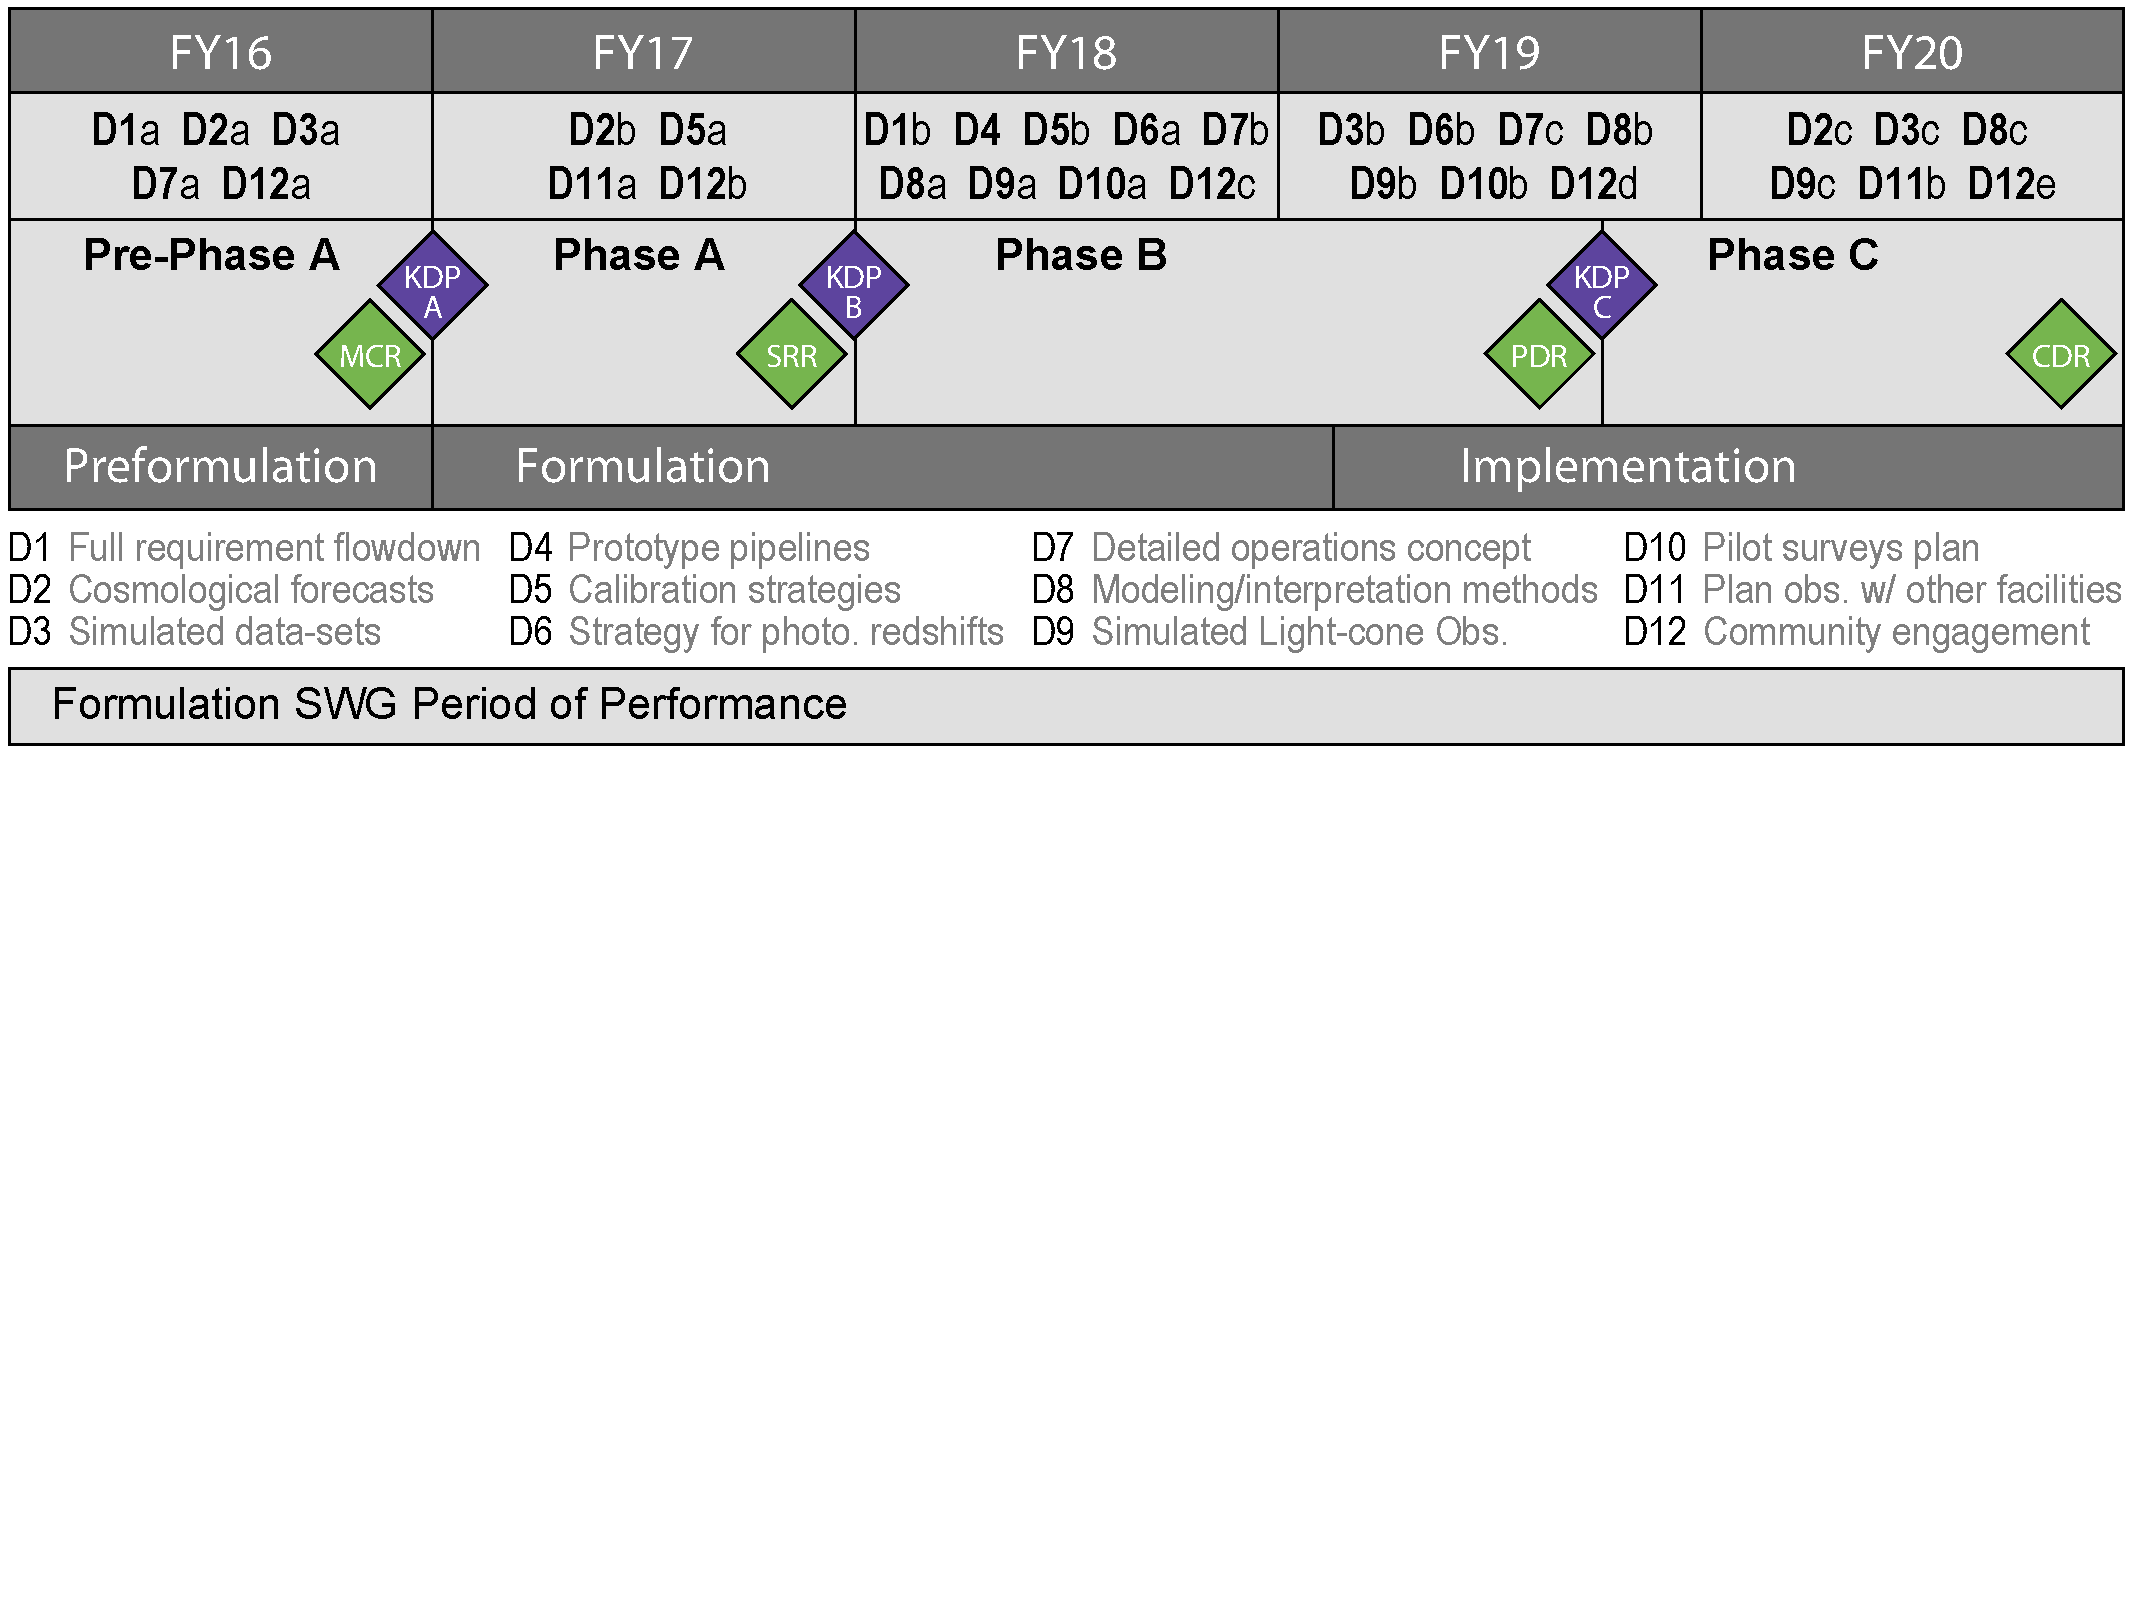
\epsfig{file=Plots/wfirst_milestones_v2.pdf,angle=0,width=0.99\textwidth}
% \end{center}
% \vspace{-0.5cm}
% \caption{{\footnotesize Our deliverable schedule in concordance with the
%       WFIRST project timeline as displayed in the WFIRST SIT call \S
%       3.2. Deliverables that are made in multiple stages are labeled
%       (a, b and c) and appear in multiple years.}}
% \label{tab:milestones_mgt}
% \end{boxedminipage}
% \end{wrapfigure}
%\end{center}
%\setlength\intextsep{0pt}
project timeline.

\subs{Postdocs and Students.}  The largest component of our budget is support for postdoctoral researchers
who will work under the supervision of the PI and Co-Is to carry out the
many calculations, simulations, and tests needed to accomplish our
tasks.  Our budget incorporates an initial plan for which postdocs will
be located at which institutions in which years to work on which tasks.

However, the optimal division of labor may shift over time, and the
Steering Committee will consider reallocations of work annually
based on internal proposals from team members.  Where appropriate,
we will consider raising collaborators to funded Co-Is, with NASA approval,
if they are best positioned to carry out particular tasks.
Many of the methodology development efforts, and some of the
technical tasks, are well suited to graduate students, supported
by other sources or by this Investigation if their work
clearly falls within its scope.  In addition to accomplishing the
work of this proposal, the involvement of many postdocs and students
will build a cadre of young researchers who are ideally positioned
to exploit the scientific opportunities of WFIRST.

\subs{A Unified Team.} As is evident from our previous discussion, jointly addressing the
weak lensing and redshift-space clustering elements of the WFIRST
dark energy program leads to an ambitious task list that offers critical
advantages relative to studying them separately.  First is the effective use of expertise; many members of
our team have expertise in both of these program elements and will
contribute to both during the course of this investigation. Second is
the commonality of the hardware; HLS Imaging and Spectroscopy use the
same telescope, detectors, and data systems, and it makes sense to develop associated requirements
through joint consideration of the two surveys.
Third is the need to develop a unified operations concept for these
two interleaved surveys; in overall footprint and in details of
dither patterns and roll angles, choices made for one survey affect
the performance of the other.

Finally, a joint investigation allows us to take a broad perspective
on the WFIRST dark energy program, including a common forecasting
framework that can account for complementary information and the
ability of one survey to mitigate systematics in the other,
common sets of cosmological simulations and models of galaxy bias
that are relevant to both topics, and investigation of trades
between HLS Imaging and Spectroscopy.  We have carefully
constructed a team capable of addressing all of the essential tasks for elements A and C of the WFIRST SIT NRA, and
we have requested resources that will enable us to accomplish this work.
If NASA decides to select additional teams in these areas we will be glad to collaborate with them.
As emphasized in \S\ref{sec:engagement}, WFIRST is a national and international resource, and
it is valuable to engage as much of the astronomical community
as possible in its formulation.
